\documentclass[oneside,11pt,a4paper,nologo]{book}

\usepackage{a4wide}

\usepackage[top=0.7in,bottom=0.7in,left=0.7in,right=0.7in]{geometry} % Page margins

% \usepackage{hyperref}

\usepackage[dvipsnames]{xcolor}
\usepackage{graphicx}
\usepackage[english]{babel}
\usepackage{varioref}
\usepackage{hyperref}
\usepackage{multicol}
\usepackage{makeidx}
\usepackage{ulem}
\usepackage{fancyhdr}
\usepackage{etoolbox}
% \usepackage{times}
\usepackage[export]{adjustbox}
\usepackage{pifont}
\usepackage{wrapfig}


% \input{pjotr_commands}

% \input{bio_commands}

%\usepackage{mathpazo} % add possibly `sc` and `osf` options
%\usepackage{eulervm}
\usepackage{palatino}
\usepackage[T1]{fontenc}

% \voffset 0pt
% \headheight 0pt
% \headsep 0pt
% \oddsidemargin 0pt

\setlength{\parindent}{0pt}                     % paragraph indent 0 pt
\setlength{\parskip}{1ex plus 0.5ex minus 0.2ex}
\setlength{\emergencystretch}{3em}              % absorb residual overfull lines (long titles/DOIs)

\newcommand{\docname}{CV}
\newcommand{\docversion}{\begin{center} $Version$ \end{center}}

\newcommand{\etal}{\emph{et~al.\ }}

\newcommand{\pprins}{{\bf {Prins~P}}}
\newcommand{\ptitle}[1]{{#1}}
\newcommand{\pyear}[1]{{ (#1) }}
\newcommand{\pvolume}[1]{\textit{#1}:}
\newcommand{\pages}[1]{{ #1}}
\newcommand{\prefs}[1]{{ (#1)}}
\newcommand{\pmid}[1]{{PMID:#1}}
\newcommand{\pmcid}[1]{{#1}}
\newcommand{\doi}[1]{DOI:{#1}}
% \newcommand{\journal}[1]{\hbox{\bf \emph{#1}}}
% \newcommand{\hijournal}[1]{{\bf \textcolor{gray}{\uline{#1}}}}
% \newcommand{\hijournal}[1]{\hbox{\bf \emph{#1}}}

\newcommand{\Rplus}{\protect\hspace{-.1em}\protect\raisebox{.3ex}{\large\textbf{+}}}
\newcommand{\fairp}{\hbox{FAIR\Rplus}}
\newcommand{\rf}[1]{\textbf{~[#1]}}

\newcommand{\wuperiodone}{October 2004 - to date}
% In dienst van/tot       : 1-10-2004 tot 1-10-2010
%                         : 4-4-2011 tot 1-11-2012
\newcommand{\rugrf}{September 2004 - to date}
\newcommand{\wufree}{June 2003 - September 2004}
\newcommand{\causadta}{August 2002 - May 2003}
\newcommand{\causperiod}{June 2000 - July 2002}
\newcommand{\specnetperiod}{May 1999 - May 2000}
\newcommand{\pacsperiod}{1998 - 1999}
\newcommand{\knpperiod}{1996 - 1998}
\newcommand{\dhakaperiod}{1993 - 1996}
\newcommand{\delftperiod}{1993 (six months)}
\newcommand{\adecsperiod}{1987 - 1992}
\newcommand{\education}{1}
\newcommand{\publications}{1}
\newcommand{\additional}{1}
\newcommand{\journal}[1]{{\bf \textcolor{NavyBlue}{#1}}}

\newcommand{\hijournal}[1]{{\bf \textcolor{NavyBlue}{\uline{#1}}}}

\renewcommand{\footrulewidth}{.6pt}             % Ruler at the bottom

\title{\docname}

\fancypagestyle{firstpage}{
\fancyhf{}                                      % empty the header and footer
% \fancyhead[LE,RO]{\slshape Page \thepage}       % pagenumber in header
% \fancyhead[LO]{\slshape \leftmark}              % leftmarker in header
% \fancyhead[RE]{\slshape \rightmark}             % rightmarker in header
\fancyfoot[LE,RO]{\today} % footer text
\fancyfoot[RE,LO]{Curriculum Vitae \\ Andrea Guarracino}
}

\fancypagestyle{plain}{
\fancyhf{}                                      % empty the header and footer
\fancyhead[LE,RO]{\slshape Page \thepage}       % pagenumber in header
\fancyhead[LO]{\slshape \leftmark}              % leftmarker in header
\fancyhead[RE]{\slshape \rightmark}             % rightmarker in header
\fancyfoot[LE,RO]{\today} % footer text
\fancyfoot[RE,LO]{Curriculum Vitae \\ Andrea Guarracino}
}

\renewcommand{\emph}[1]{{\it #1}}

\newcommand{\bibhref}[1]{\href{#1}{\ding{234}}}
\newcommand{\pacs}{\emph{PACS}}
\newcommand{\unix}{\emph{UNIX}}
\newcommand{\linux}{\emph{Linux}}
\newcommand{\rockl}{\emph{ROCK Linux}}
\newcommand{\windows}{\emph{Microsoft Windows}}
\newcommand{\solaris}{\emph{Solaris}}
\newcommand{\mis}{\emph{MIS}}
\newcommand{\cad}{\emph{CAD}}

% Languages

\newcommand{\java}{\emph{JAVA}}
\newcommand{\ejb}{\emph{EJB}}
\newcommand{\cpp}{\emph{C++}}
\newcommand{\perl}{\emph{Perl}}
\newcommand{\ruby}{\emph{Ruby}}

% Design

\newcommand{\oop}{\emph{OOP}}
\newcommand{\uml}{\emph{UML}}
\newcommand{\rup}{\emph{RUP}}
\newcommand{\xp}{\emph{XP}}

% Tools

\newcommand{\cfengine}{\emph{CFEngine}}
\newcommand{\bash}{\emph{bash}}

% Protocols

\newcommand{\tcpip}{\emph{TCP/IP}}
\newcommand{\http}{\emph{HTTP}}
\newcommand{\udp}{\emph{UDP}}
\newcommand{\ssl}{\emph{SSL}}
\newcommand{\xml}{\emph{XML}}
\newcommand{\rug}{RUG}
\newcommand{\wu}{WU}


\AtBeginDocument{\pagestyle{firstpage}}

\date{\today}
\author{CV - Andrea Guarracino}

\begin{document}

\setcounter{page}{1}




\begin{figure}
    \centering
    \begin{minipage}{0.45\textwidth}
        \centering
        
\includegraphics[width=0.9\textwidth]{AndreaGuarracinoPhoto} % first figure itself
        % \caption{first figure}
    \end{minipage}\hfill
    \begin{minipage}{0.45\textwidth}
        \centering
        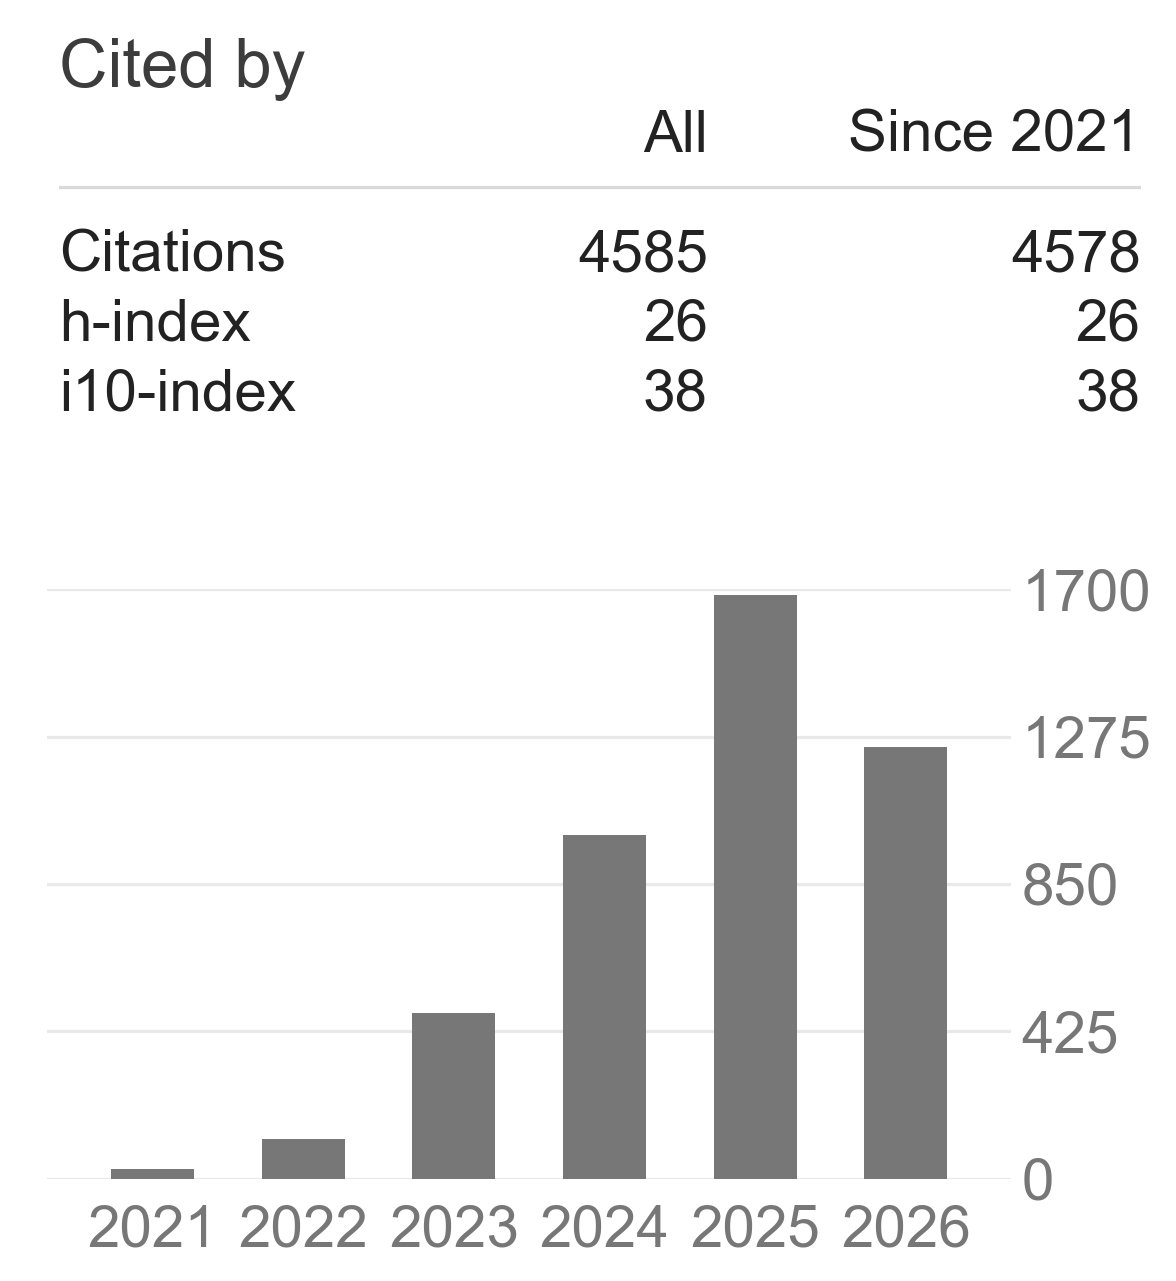
\includegraphics[width=0.9\textwidth]{AndreaGuarracinoGoogleScholar} % second figure itself
        % \caption{Google Scholar}
    \end{minipage}
\end{figure}

% }

% \vspace{-1.3in}

% \small
\section*{Andrea Guarracino}

% \footnote{Repeating note}

\begin{tabular}{p{5cm}l}  % column alignment r=right l=left c=center
  Surname, Name & \uline{Guarracino}, Andrea \\
  Job title       & Assistant Professor \\
  Department      & Bioinnovation and Genome Sciences Division \\
  & Translational Genomics Research Institute (TGen) \\
  & 445 N 5th Street, Phoenix, AZ, 85004, USA \\
  % Cell            & (+XX) XXXXXXX (IT) \\
  E-mail          & aguarracino@tgen.org \\
  % Date of birth   & XX XXXX XXXX \\
  % Marital status  & Single \\
  Nationality     & Italian (IT) \\
  % Tax Code        & XXXXXXX \\
  % Previous Job title & `Postdoctoral Scholar at the UTHSC (Memphis, USA) \\
  Web site \& publications & https://andreaguarracino.github.io/~\href{https://andreaguarracino.github.io/}{\ding{234}} \\
  Projects \& source code & https://github.com/AndreaGuarracino~\href{https://github.com/AndreaGuarracino}{\ding{234}} \\
  ORCID & 0000-0001-9744-131X~\href{https://orcid.org/0000-0001-9744-131X}{\ding{234}} \\
  % Peer reviewed publications & XX \\
  Publications & {\bf 40} peer reviewed + {\bf 12} preprints = {\bf 52} total ({\bf 10} first or last)~\href{http://www.ncbi.nlm.nih.gov/pubmed/?term=Andrea+Guarracino[Author]}{\ding{234}} \\
  Google Scholar & Citations 4585 (July 2026)~\href{https://scholar.google.com/citations?user=zABbjIoAAAAJ&hl=en}{\ding{234}} \\
\end{tabular}


\ifdef{\education}{

\subsection*{Degrees}

Ph.D. (2022) \emph{Investigating chromosomal instability in cancer stem cells}, Cellular and Molecular Biology (Bioinformatics), University of Rome Tor Vergata, Italy

M.Sc. (2018) \emph{Energetic and functional characterization of phosphorylations involved in the co-regulation of protein interaction}, Bioinformatics (LM-6), University of Rome Tor Vergata, Italy

B.Sc. (2010) \emph{High Dynamic Range (HDR) methods for industrial inspection applications}, Computer Engineering (L-8), University of Salerno, Italy

} % education

\subsection*{Professional experience}

% \begin{tabular}{p{2cm}p{12.3cm}}  % column alignment r=right l=left c=center
\begin{tabular}{p{2cm}p{12.3cm}}  % column alignment r=right l=left c=center
    2026---  & Assistant Professor, Bioinnovation and Genome Sciences Division, Translational Genomics Research Institute (TGen), Phoenix, AZ, USA \\

    2025---2025  & Assistant Professor, Dept.\ of Genetics, Genomics \& Informatics, University of Tennessee Health Science Center, Memphis, USA \\

    2023---  & Honorary contract holder, Princess Máxima Center for Pediatric Oncology, Utrecht, Netherlands \\

    2022---  & E-Visitor, Human Technopole, Milan, Italy \\

    2022---2025  & Postdoctoral Scholar, Dept.\ of Genetics, Genomics \& Informatics, University of Tennessee Health Science Center, Memphis, USA \\

    2021---2022  & Postdoctoral Associate, Human Technopole, Milan, Italy \\

    2019---  & Research collaborator, Italian Institute for Genomic Medicine \& Candiolo Cancer Institute, Italy \\

    2018---2022  & Ph.D. student, Dept.\ of Cellular and Molecular Biology, University of Rome Tor Vergata, Rome, Italy \\

    2013---2018  & Computer engineer, GISA S.n.c., Salerno, Italy \\

    2012---2013 & Salesman, L'Erborista S.A.S.\ di Sarno Adele \& C, Salerno, Italy \\

    2010---2012  & Web Developer, Virtual, Salerno, Italy \\
    \end{tabular}

% \end{tabular}

\subsection*{Awards}

2020 \emph{Best Poster Prize} on ``Semantic Variation Graphs: Ontologies for Pangenome Graphs'', ISMB~\href{https://www.iscb.org/ismb2020-general/ismb2020-award-winners\#bio-poster}{\ding{234}}

2016--2018 Scholarships during the Master’s degree in Bioinformatics, University of Rome Tor Vergata, Italy

2007--2010 Scholarships during the Bachelor’s degree in Computer Engineering, University of Salerno, Italy




\ifdef{\publications}{

\subsection*{Publications}

% \begin{enumerate}
\begin{enumerate}
\item Hansen NF, Dwarshuis N, Ji HJ, ..., \textbf{Guarracino A} \emph{et al.}\pyear{In press}\ptitle{A complete diploid human genome benchmark for personalized genomics}. \ \hijournal{Cell}  \ \prefs{\pmcid{PMC12458380}, \pmid{41000953}, \doi{10.\allowbreak{}1101/\allowbreak{}2025.\allowbreak{}09.\allowbreak{}21.\allowbreak{}677443}~\href{https://doi.org/10.1101/2025.09.21.677443}{\ding{234}}}
\item Darnell SS, Overall RW, \textbf{Guarracino A}, Colonna V, Villani F, Garrison E, Isaac A, Muli P \emph{et al.}\pyear{2025}\ptitle{Creating a biomedical knowledge base by addressing GPT inaccurate responses and benchmarking context}. \ \journal{Open Research Africa}  \ \prefs{\doi{10.\allowbreak{}12688/\allowbreak{}openresafrica.\allowbreak{}15854.\allowbreak{}1}~\href{https://doi.org/10.12688/openresafrica.15854.1}{\ding{234}}}
\item Edwards SV, Fang B, Khost D, ..., \textbf{Guarracino A} \emph{et al.}\pyear{2025}\ptitle{Multispecies pangenomes reveal a pervasive influence of population size on structural variation}. \ \hijournal{Science} \pvolume{390} \ \prefs{\pmcid{PMC13295103}, \pmid{41379974}, \doi{10.\allowbreak{}1126/\allowbreak{}science.\allowbreak{}adw1931}~\href{https://doi.org/10.1126/science.adw1931}{\ding{234}}}
\item Kronenberg Z, Nolan C, Porubsky D, ..., \textbf{Guarracino A} \emph{et al.}\pyear{2025}\ptitle{The Platinum Pedigree: a long-read benchmark for genetic variants}. \ \hijournal{Nature Methods}  \ \prefs{\pmcid{PMC12533576}, \pmid{40759746}, \doi{10.\allowbreak{}1038/\allowbreak{}s41592-025-02750-y}~\href{https://doi.org/10.1038/s41592-025-02750-y}{\ding{234}}}
\item Gomes de Lima L*, \textbf{Guarracino A*}, Koren S*, Potapova T, McKinney S, Rhie A, Solar SJ, Seidel C \emph{et al.}\pyear{2025}\ptitle{The formation and propagation of human Robertsonian chromosomes}. \ \hijournal{Nature}  \ \prefs{\pmcid{PMC12657243}, \pmid{40993387}, \doi{10.\allowbreak{}1038/\allowbreak{}s41586-025-09540-8}~\href{https://doi.org/10.1038/s41586-025-09540-8}{\ding{234}}}
\item Porubsky D, Dashnow H, Sasani TA, ..., \textbf{Guarracino A} \emph{et al.}\pyear{2025}\ptitle{Human de novo mutation rates from a four-generation pedigree reference}. \ \hijournal{Nature}  \ \prefs{\pmcid{PMC12240836}, \pmid{40269156}, \doi{10.\allowbreak{}1038/\allowbreak{}s41586-025-08922-2}~\href{https://doi.org/10.1038/s41586-025-08922-2}{\ding{234}}}
\item Yoo D, Rhie A, Hebbar P, ..., \textbf{Guarracino A} \emph{et al.}\pyear{2025}\ptitle{Complete sequencing of ape genomes}. \ \hijournal{Nature}  \ \prefs{\pmcid{PMC12058530}, \pmid{40205052}, \doi{10.\allowbreak{}1038/\allowbreak{}s41586-025-08816-3}~\href{https://doi.org/10.1038/s41586-025-08816-3}{\ding{234}}}
\item Cheng L, Wang N, Bao Z, Zhou Q, \textbf{Guarracino A}, Yang Y, Wang P, Zhang Z \emph{et al.}\pyear{2025}\ptitle{Leveraging a phased pangenome for haplotype design of hybrid potato}. \ \hijournal{Nature}  \ \prefs{\pmcid{PMC11981936}, \pmid{39843749}, \doi{10.\allowbreak{}1038/\allowbreak{}s41586-024-08476-9}~\href{https://doi.org/10.1038/s41586-024-08476-9}{\ding{234}}}
\item Corda L, Volpe E, Dallali H, Di Tommaso E, Colantoni A, \textbf{Guarracino A}, Chittoor SS, Capulli M \emph{et al.}\pyear{2025}\ptitle{Cell line-matched reference enables high-precision functional genomics}. \ \hijournal{Nature Communications}  \ \prefs{\pmcid{PMC12711918}, \pmid{41266327}, \doi{10.\allowbreak{}1038/\allowbreak{}s41467-025-66155-3}~\href{https://doi.org/10.1038/s41467-025-66155-3}{\ding{234}}}
\item Volpe E, Colantoni A, Corda L, Di Tommaso E, Pelliccia F, Ottalevi R, \textbf{Guarracino A}, Licastro D \emph{et al.}\pyear{2025}\ptitle{The reference genome of the human diploid cell line RPE-1}. \ \hijournal{Nature Communications} \pvolume{16} \ \prefs{\pmcid{PMC12432231}, \pmid{40940351}, \doi{10.\allowbreak{}1038/\allowbreak{}s41467-025-62428-z}~\href{https://doi.org/10.1038/s41467-025-62428-z}{\ding{234}}}
\item Helmy M, Li JU, Yan XF, ..., \textbf{Guarracino A} \emph{et al.}\pyear{2025}\ptitle{High-quality mouse reference genomes reveal the structural complexity of the murine protein-coding landscape}. \ \hijournal{Cell Genomics} \pages{101074} \ \prefs{\pmcid{PMC12903361}, \pmid{41330379}, \doi{10.\allowbreak{}1016/\allowbreak{}j.\allowbreak{}xgen.\allowbreak{}2025.\allowbreak{}101074}~\href{https://doi.org/10.1016/j.xgen.2025.101074}{\ding{234}}}
\item Potapova TA, Kostos P, McKinney S, Borchers M, Haug J, \textbf{Guarracino A}, Solar SJ, Mattingly M \emph{et al.}\pyear{2025}\ptitle{Chromosome-specific epigenetic control and transmission of ribosomal DNA arrays in Hominidae genomes}. \ \hijournal{Cell Genomics} \pages{101031} \ \prefs{\pmcid{PMC12802695}, \pmid{41043432}, \doi{10.\allowbreak{}1016/\allowbreak{}j.\allowbreak{}xgen.\allowbreak{}2025.\allowbreak{}101031}~\href{https://doi.org/10.1016/j.xgen.2025.101031}{\ding{234}}}
\item Li L, Wu Z, \textbf{Guarracino A}, Villani F, Kong D, Mancieri A, Zhang A, Saba L \emph{et al.}\pyear{2025}\ptitle{Genetic modulation of protein expression in rat brain}. \ \journal{iScience} \pvolume{28}\pages{112079} \ \prefs{\pmcid{PMC11930185}, \pmid{40124499}, \doi{10.\allowbreak{}1016/\allowbreak{}j.\allowbreak{}isci.\allowbreak{}2025.\allowbreak{}112079}~\href{https://doi.org/10.1016/j.isci.2025.112079}{\ding{234}}}
\item Villani F, \textbf{Guarracino A}, Ward RR, Green T, Emms M, Pravenec M, Sharp B, Prins P \emph{et al.}\pyear{2025}\ptitle{Pangenome reconstruction in rats enhances genotype-phenotype mapping and variant discovery}. \ \journal{iScience} \pages{111835} \ \prefs{\pmcid{PMC11875200}, \pmid{40034122}, \doi{10.\allowbreak{}1016/\allowbreak{}j.\allowbreak{}isci.\allowbreak{}2025.\allowbreak{}111835}~\href{https://doi.org/10.1016/j.isci.2025.111835}{\ding{234}}}
\item Li J, Schmelzle JN, Du Y, Heumos S, \textbf{Guarracino A}, Guidi G, Prins P, Garrison E \emph{et al.}\pyear{2024}\ptitle{Rapid GPU-Based Pangenome Graph Layout}. \ \journal{SC24 (IEEE)} \pages{1-19} \ \prefs{\doi{10.\allowbreak{}1109/\allowbreak{}sc41406.\allowbreak{}2024.\allowbreak{}00035}~\href{https://doi.org/10.1109/sc41406.2024.00035}{\ding{234}}}
\item Koren S, Bao Z, \textbf{Guarracino A}, Ou S, Goodwin S, Jenike KM, Lucas J, McNulty B \emph{et al.}\pyear{2024}\ptitle{Gapless assembly of complete human and plant chromosomes using only nanopore sequencing}. \ \journal{Genome Research}  \ \prefs{\pmcid{PMC11610574}, \pmid{39505490}, \doi{10.\allowbreak{}1101/\allowbreak{}gr.\allowbreak{}279334.\allowbreak{}124}~\href{https://doi.org/10.1101/gr.279334.124}{\ding{234}}}
\item Gustafson JA, Gibson SB, Damaraju N, ..., \textbf{Guarracino A} \emph{et al.}\pyear{2024}\ptitle{High-coverage nanopore sequencing of samples from the 1000 Genomes Project to build a comprehensive catalog of human genetic variation}. \ \journal{Genome Research} \pages{gr.279273.124} \ \prefs{\pmcid{PMC11610458}, \pmid{39358015}, \doi{10.\allowbreak{}1101/\allowbreak{}gr.\allowbreak{}279273.\allowbreak{}124}~\href{https://doi.org/10.1101/gr.279273.124}{\ding{234}}}
\item Buqué A, Bloy N, Petroni G, ..., \textbf{Guarracino A} \emph{et al.}\pyear{2024}\ptitle{Impact of radiation therapy dose, fractionation, and immunotherapeutic partner in a mouse model of hormone receptor-positive mammary carcinogenesis}. \ \journal{JNCI: Journal of the National Cancer Institute}  \ \prefs{\pmcid{PMC12058254}, \pmid{39661487}, \doi{10.\allowbreak{}1093/\allowbreak{}jnci/\allowbreak{}djae329}~\href{https://doi.org/10.1093/jnci/djae329}{\ding{234}}}
\item Heumos S, Heuer ML, Hanssen F, Heumos L, \textbf{Guarracino A}, Heringer P, Ehmele P, Prins P \emph{et al.}\pyear{2024}\ptitle{Cluster-efficient pangenome graph construction with nf-core/pangenome}. \ \journal{Bioinformatics}  \ \prefs{\pmcid{PMC11568064}, \pmid{39400346}, \doi{10.\allowbreak{}1093/\allowbreak{}bioinformatics/\allowbreak{}btae609}~\href{https://doi.org/10.1093/bioinformatics/btae609}{\ding{234}}}
\item Heumos S*, \textbf{Guarracino A*}, Schmelzle JNM, Li J, Zhang Z, Hagmann J, Nahnsen S, Prins P \emph{et al.}\pyear{2024}\ptitle{Pangenome graph layout by Path-Guided Stochastic Gradient Descent}. \ \hijournal{Bioinformatics} \pages{btae363} \ \prefs{\pmcid{PMC11227364}, \pmid{38960860}, \doi{10.\allowbreak{}1093/\allowbreak{}bioinformatics/\allowbreak{}btae363}~\href{https://doi.org/10.1093/bioinformatics/btae363}{\ding{234}}}
\item Garrison E*, \textbf{Guarracino A*}, Heumos S, Villani F, Bao Z, Tattini L, Hagmann J, Vorbrugg S \emph{et al.}\pyear{2024}\ptitle{Building pangenome graphs}. \ \hijournal{Nature Methods}  \ \prefs{\pmid{39433878}, \doi{10.\allowbreak{}1038/\allowbreak{}s41592-024-02430-3}~\href{https://doi.org/10.1038/s41592-024-02430-3}{\ding{234}}}
\item Bolognini D, Halgren A, Lou RN, Raveane A, Rocha JL, \textbf{Guarracino A}, Soranzo N, Chin CS \emph{et al.}\pyear{2024}\ptitle{Recurrent evolution and selection shape structural diversity at the amylase locus}. \ \hijournal{Nature}  \ \prefs{\pmcid{PMC11485256}, \pmid{39232174}, \doi{10.\allowbreak{}1038/\allowbreak{}s41586-024-07911-1}~\href{https://doi.org/10.1038/s41586-024-07911-1}{\ding{234}}}
\item Yang Z, \textbf{Guarracino A}, Biggs PJ, Black MA, Ismail N, Wold JR, Merriman TR, Prins P \emph{et al.}\pyear{2023}\ptitle{Pangenome graphs in infectious disease: a comprehensive genetic variation analysis of Neisseria meningitidis leveraging Oxford Nanopore long reads}. \ \hijournal{Frontiers in Genetics} \pvolume{14} \ \prefs{\pmcid{PMC10448961}, \pmid{37636268}, \doi{10.\allowbreak{}3389/\allowbreak{}fgene.\allowbreak{}2023.\allowbreak{}1225248}~\href{https://doi.org/10.3389/fgene.2023.1225248}{\ding{234}}}
\item Cochetel N, Minio A, \textbf{Guarracino A}, Garcia JF, Figueroa-Balderas R, Massonnet M, Kasuga T, Londo JP \emph{et al.}\pyear{2023}\ptitle{A super-pangenome of the North American wild grape species}. \ \hijournal{Genome Biology} \pvolume{24} \ \prefs{\pmcid{PMC10729490}, \pmid{38111050}, \doi{10.\allowbreak{}1186/\allowbreak{}s13059-023-03133-2}~\href{https://doi.org/10.1186/s13059-023-03133-2}{\ding{234}}}
\item Marco-Sola S, Eizenga JM, \textbf{Guarracino A}, Paten B, Garrison E, Moreto M\pyear{2023}\ptitle{Optimal gap-affine alignment in O(s) space}. \ \hijournal{Bioinformatics}  \ \prefs{\pmcid{PMC9940620}, \pmid{36749013}, \doi{10.\allowbreak{}1093/\allowbreak{}bioinformatics/\allowbreak{}btad074}~\href{https://doi.org/10.1093/bioinformatics/btad074}{\ding{234}}}
\item Rhie A, Nurk S, Cechova M, ..., \textbf{Guarracino A} \emph{et al.}\pyear{2023}\ptitle{The complete sequence of a human Y chromosome}. \ \hijournal{Nature} \pvolume{621}\pages{344--354} \ \prefs{\pmcid{PMC10752217}, \pmid{37612512}, \doi{10.\allowbreak{}1038/\allowbreak{}s41586-023-06457-y}~\href{https://doi.org/10.1038/s41586-023-06457-y}{\ding{234}}}
\item \textbf{Guarracino A*}, Buonaiuto S, de Lima LG, Potapova T, Rhie A, Koren S, Rubinstein B, Fischer C \emph{et al.}\pyear{2023}\ptitle{Recombination between heterologous human acrocentric chromosomes}. \ \hijournal{Nature} \pvolume{617}\pages{335--343} \ \prefs{\pmcid{PMC10172130}, \pmid{37165241}, \doi{10.\allowbreak{}1038/\allowbreak{}s41586-023-05976-y}~\href{https://doi.org/10.1038/s41586-023-05976-y}{\ding{234}}}
\item Liao WW, Asri M, Ebler J, ..., \textbf{Guarracino A} \emph{et al.}\pyear{2023}\ptitle{A draft human pangenome reference}. \ \hijournal{Nature} \pvolume{617}\pages{312--324} \ \prefs{\pmcid{PMC10172123}, \pmid{37165242}, \doi{10.\allowbreak{}1038/\allowbreak{}s41586-023-05896-x}~\href{https://doi.org/10.1038/s41586-023-05896-x}{\ding{234}}}
\item Garrison E and \textbf{Guarracino A}\pyear{2022}\ptitle{Unbiased pangenome graphs}. \ \hijournal{Bioinformatics}  \ \prefs{\pmcid{PMC9805579}, \pmid{36448683}, \doi{10.\allowbreak{}1093/\allowbreak{}bioinformatics/\allowbreak{}btac743}~\href{https://doi.org/10.1093/bioinformatics/btac743}{\ding{234}}}
\item \textbf{Guarracino A*}, Heumos S*, Nahnsen S, Prins P, Garrison E\pyear{2022}\ptitle{ODGI: understanding pangenome graphs}. \ \hijournal{Bioinformatics}  \ \prefs{\pmcid{PMC9237687}, \pmid{35552372}, \doi{10.\allowbreak{}1093/\allowbreak{}bioinformatics/\allowbreak{}btac308}~\href{https://doi.org/10.1093/bioinformatics/btac308}{\ding{234}}}
\item Musella M, \textbf{Guarracino A}, Manduca N, Galassi C, Ruggiero E, Potenza A, Maccafeo E, Manic G \emph{et al.}\pyear{2022}\ptitle{Type I IFNs promote cancer cell stemness by triggering the epigenetic regulator KDM1B}. \ \hijournal{Nature Immunology}  \ \prefs{\pmcid{PMC9477743}, \pmid{36002648}, \doi{10.\allowbreak{}1038/\allowbreak{}s41590-022-01290-3}~\href{https://doi.org/10.1038/s41590-022-01290-3}{\ding{234}}}
\item Jarvis ED, Formenti G, Rhie A, \textbf{Guarracino A}, Yang C, Wood J, Tracey A, Thibaud-Nissen F \emph{et al.}\pyear{2022}\ptitle{Semi-automated assembly of high-quality diploid human reference genomes}. \ \hijournal{Nature}  \ \prefs{\pmcid{PMC9668749}, \pmid{36261518}, \doi{10.\allowbreak{}1038/\allowbreak{}s41586-022-05325-5}~\href{https://doi.org/10.1038/s41586-022-05325-5}{\ding{234}}}
\item Pepe G, \textbf{Guarracino A}, Ballesio F, Parca L, Ausiello G, Helmer-Citterich M\pyear{2022}\ptitle{Evaluation of potential miRNA sponge effects of SARS genomes in human}. \ \hijournal{Non-coding RNA Research} \pvolume{7}\pages{48--53} \ \prefs{\pmcid{PMC8769905}, \pmid{35075440}, \doi{10.\allowbreak{}1016/\allowbreak{}j.\allowbreak{}ncrna.\allowbreak{}2022.\allowbreak{}01.\allowbreak{}003}~\href{https://doi.org/10.1016/j.ncrna.2022.01.003}{\ding{234}}}
\item Mattiello L, Abdel Rehim SS, Musella M, Sistigu A, \textbf{Guarracino A}, Vitale S, Corradi F, Galassi C \emph{et al.}\pyear{2021}\ptitle{The Targeting of MRE11 or RAD51 Sensitizes Colorectal Cancer Stem Cells to CHK1 Inhibition}. \ \hijournal{Cancers} \pvolume{13}\pages{1957} \ \prefs{\pmcid{PMC8073980}, \pmid{33921638}, \doi{10.\allowbreak{}3390/\allowbreak{}cancers13081957}~\href{https://doi.org/10.3390/cancers13081957}{\ding{234}}}
\item Marco P*, Adinolfi M*, \textbf{Guarracino A*}, Ferrè F, Ausiello G, Vitale I, Helmer-Citterich M\pyear{2021}\ptitle{Relative Information Gain: Shannon entropy-based measure of the relative structural conservation in RNA alignments}. \ \hijournal{NAR Genomics and Bioinformatics} \pvolume{3} \ \prefs{\pmcid{PMC7884220}, \pmid{33615214}, \doi{10.\allowbreak{}1093/\allowbreak{}nargab/\allowbreak{}lqab007}~\href{https://doi.org/10.1093/nargab/lqab007}{\ding{234}}}
\item \textbf{Guarracino A*}, Pepe G*, Ballesio F, Adinolfi M, Pietrosanto M, Sangiovanni E, Vitale I, Ausiello G \emph{et al.}\pyear{2021}\ptitle{BRIO: a web server for RNA sequence and structure motif scan}. \ \hijournal{Nucleic Acids Research}  \ \prefs{\pmcid{PMC8262756}, \pmid{34038531}, \doi{10.\allowbreak{}1093/\allowbreak{}nar/\allowbreak{}gkab400}~\href{https://doi.org/10.1093/nar/gkab400}{\ding{234}}}
\item Ferrarini MG, Lal A, Rebollo R, Gruber AJ, \textbf{Guarracino A}, Gonzalez IM, Floyd T, de Oliveira DS \emph{et al.}\pyear{2021}\ptitle{Genome-wide bioinformatic analyses predict key host and viral factors in SARS-CoV-2 pathogenesis}. \ \hijournal{Communications Biology} \pvolume{4}\pages{590} \ \prefs{\pmcid{PMC8128904}, \pmid{34002013}, \doi{10.\allowbreak{}1038/\allowbreak{}s42003-021-02095-0}~\href{https://doi.org/10.1038/s42003-021-02095-0}{\ding{234}}}
\item Novelli G, Liu J, Biancolella M, ..., \textbf{Guarracino A} \emph{et al.}\pyear{2021}\ptitle{Inhibition of HECT E3 ligases as potential therapy for COVID-19}. \ \hijournal{Cell Death \& Disease} \pvolume{12}\pages{1--18} \ \prefs{\pmcid{PMC7987752}, \pmid{33762578}, \doi{10.\allowbreak{}1038/\allowbreak{}s41419-021-03513-1}~\href{https://doi.org/10.1038/s41419-021-03513-1}{\ding{234}}}
\item Manic G, Musella M, Corradi F, ..., \textbf{Guarracino A} \emph{et al.}\pyear{2021}\ptitle{Control of replication stress and mitosis in colorectal cancer stem cells through the interplay of PARP1, MRE11 and RAD51}. \ \hijournal{Cell Death \& Differentiation} \pages{1--23} \ \prefs{\pmcid{PMC8257675}, \pmid{33531658}, \doi{10.\allowbreak{}1038/\allowbreak{}s41418-020-00733-4}~\href{https://doi.org/10.1038/s41418-020-00733-4}{\ding{234}}}
\end{enumerate}

% \end{enumerate}

}

\subsection*{Preprints}

% \begin{enumerate}
\begin{enumerate}
\item Lucas JK, Hebbar P, Liao WW, ..., \textbf{Guarracino A} \emph{et al.}\pyear{Submitted}\ptitle{HPRC2: A human pangenome reference with near-complete coverage of common genetic variation}. \ \journal{bioRxiv}  \ \prefs{\doi{10.\allowbreak{}64898/\allowbreak{}2026.\allowbreak{}07.\allowbreak{}21.\allowbreak{}739710}~\href{https://doi.org/10.64898/2026.07.21.739710}{\ding{234}}}
\item Shih PJ, Sanghani Z, \textbf{Guarracino A}, Gamaarachchi H, Batten C\pyear{Submitted}\ptitle{Panomap: Unbiased Nanopore Signal Mapping with Pangenome Variation Graphs}. \ \journal{bioRxiv}  \ \prefs{\doi{10.\allowbreak{}64898/\allowbreak{}2026.\allowbreak{}07.\allowbreak{}10.\allowbreak{}737796}~\href{https://doi.org/10.64898/2026.07.10.737796}{\ding{234}}}
\item \textbf{Guarracino A*}, Gyamfi A, Human Pangenome Reference Consortium, Garrison E\pyear{Submitted}\ptitle{Concerted evolution and unorthodox recombination of human subtelomeres}. \ \journal{bioRxiv}  \ \prefs{\pmcid{PMC13370367}, \pmid{42465281}, \doi{10.\allowbreak{}64898/\allowbreak{}2026.\allowbreak{}07.\allowbreak{}10.\allowbreak{}737660}~\href{https://doi.org/10.64898/2026.07.10.737660}{\ding{234}}}
\item Formenti G, Absolon DE, Abueg LAL, ..., \textbf{Guarracino A} \emph{et al.}\pyear{Submitted}\ptitle{The Vertebrate Genomes Project Phase I: A global reference genome resource}. \ \journal{bioRxiv}  \ \prefs{\pmcid{PMC13320880}, \pmid{42395566}, \doi{10.\allowbreak{}64898/\allowbreak{}2026.\allowbreak{}06.\allowbreak{}24.\allowbreak{}732306}~\href{https://doi.org/10.64898/2026.06.24.732306}{\ding{234}}}
\item Rocha J, Lou RN, De Lima Adam C, ..., \textbf{Guarracino A} \emph{et al.}\pyear{Submitted}\ptitle{A Pan-pangenome illuminates complex structural variation and selection in humans, chimpanzees, and bonobos}. \ \journal{bioRxiv}  \ \prefs{\pmcid{PMC13277932}, \pmid{42327276}, \doi{10.\allowbreak{}64898/\allowbreak{}2026.\allowbreak{}06.\allowbreak{}06.\allowbreak{}730619}~\href{https://doi.org/10.64898/2026.06.06.730619}{\ding{234}}}
\item Hallast P, Rhie A, Loftus M, ..., \textbf{Guarracino A} \emph{et al.}\pyear{Submitted}\ptitle{Population-scale Y chromosome assemblies reveal recurrent remodeling within constrained architectures}. \ \journal{bioRxiv}  \ \prefs{\pmcid{PMC13252187}, \pmid{42282846}, \doi{10.\allowbreak{}64898/\allowbreak{}2026.\allowbreak{}06.\allowbreak{}03.\allowbreak{}729890}~\href{https://doi.org/10.64898/2026.06.03.729890}{\ding{234}}}
\item Ranallo-Benavidez TR, Chen YA, Potapova TA, Alanko JN, Loucks H, Lucas J, Human Pangenome Reference Consortium, \textbf{Guarracino A} \emph{et al.}\pyear{Submitted}\ptitle{KaryoScope: rapid, alignment-free sequence annotation for the pangenome era}. \ \journal{bioRxiv}  \ \prefs{\doi{10.\allowbreak{}64898/\allowbreak{}2026.\allowbreak{}05.\allowbreak{}15.\allowbreak{}725544}~\href{https://doi.org/10.64898/2026.05.15.725544}{\ding{234}}}
\item Wagner J, Keskus AG, Oshima KK, ..., \textbf{Guarracino A} \emph{et al.}\pyear{Submitted}\ptitle{A complete human pancreatic cancer genome}. \ \journal{bioRxiv}  \ \prefs{\pmcid{PMC13174521}, \pmid{42146349}, \doi{10.\allowbreak{}64898/\allowbreak{}2026.\allowbreak{}05.\allowbreak{}01.\allowbreak{}722316}~\href{https://doi.org/10.64898/2026.05.01.722316}{\ding{234}}}
\item Kaushan H, Marco-Sola S, Garrison E, Prins P, \textbf{Guarracino A**}\pyear{Submitted}\ptitle{Adaptive Tracepoints for Pangenome Alignment Compression}. \ \journal{bioRxiv}  \ \prefs{\pmcid{PMC12934660}, \pmid{41757015}, \doi{10.\allowbreak{}64898/\allowbreak{}2026.\allowbreak{}02.\allowbreak{}16.\allowbreak{}706236}~\href{https://doi.org/10.64898/2026.02.16.706236}{\ding{234}}}
\item Bolognini D*, \textbf{Guarracino A*}, Paleni C, Dudley TS, Iacoviello L, Raveane A, Sudmant PH, Garrison E \emph{et al.}\pyear{Submitted}\ptitle{Population-scalable genotyping from low-coverage sequencing data using pangenome graphs}. \ \journal{bioRxiv}  \ \prefs{\doi{10.\allowbreak{}64898/\allowbreak{}2026.\allowbreak{}02.\allowbreak{}05.\allowbreak{}704023}~\href{https://doi.org/10.64898/2026.02.05.704023}{\ding{234}}}
\item Solar SJ, Hebbar P, de Lima LG, Sweeten AP, Rhie A, Potapova TA, de Gennaro L, \textbf{Guarracino A} \emph{et al.}\pyear{Submitted}\ptitle{Origin and evolution of acrocentric chromosomes in human and great apes}. \ \journal{bioRxiv}  \ \prefs{\pmcid{PMC12767296}, \pmid{41497641}, \doi{10.\allowbreak{}64898/\allowbreak{}2025.\allowbreak{}12.\allowbreak{}22.\allowbreak{}696095}~\href{https://doi.org/10.64898/2025.12.22.696095}{\ding{234}}}
\item Obinu L, \textbf{Guarracino A}, Trivedi U, Porceddu A\pyear{Submitted}\ptitle{The reference-free pangenome of Arabidopsis thaliana}. \ \journal{bioRxiv}  \ \prefs{\doi{10.\allowbreak{}1101/\allowbreak{}2025.\allowbreak{}06.\allowbreak{}25.\allowbreak{}661508}~\href{https://doi.org/10.1101/2025.06.25.661508}{\ding{234}}}
\end{enumerate}

% \end{enumerate}


\subsection*{Educational activities}

\begin{tabular}{p{2cm}p{12.3cm}}  % column alignment r=right l=left c=center
  \textbf{Ongoing} & \\


  2023--- & Advisor of PhD student Giada Sancamillo, SEMM European School of Molecular Medicine (Italy), "Dissecting the intracellular response to replication and mitotic stress in colorectal cancer for the design of novel effective (immuno)therapies" \\

  \textbf{Past} & \\
  2024---2025 & Advisor of masters student Ludovica Perticone, University of Rome Tor Vergata (Italy), "Benchmarking Analytical Pipelines for Single-Cell Long-Read Sequencing in Colon Cancer" \\

  2021---2022 & Advisor of masters student Simone Campagna, University of Rome Tor Vergata (Italy), "Machine learning to automatically detect the \textit{C. elegans} bodies from microscope images and measure their growth over time" \\

  2021 & Supervisor of bachelors student Alessandro Pucci, University of Rome Tor Vergata (Italy), "Analysis of the effect of SARS-CoV-2 mutations on the pairing between the viral genome and human miRNAs" \\

  2020---2021 & Supervisor of masters student Tiziano Tomarelli, University of Rome Tor Vergata (Italy), "Machine Learning methods applied to kinase-substrate interaction prediction" \\
  
  2020 & Supervisor of masters student Federico Spettich, University of Rome Tor Vergata (Italy), "Natural Language Processing techniques for protein encoding applied to phosphorylation prediction" \\

  2020 & Supervisor of bachelors student Chiara Notturno, University of Rome Tor Vergata (Italy), "Analysis of repeated sequences in lincRNA candidates for exon shuffling" \\

  2019---2020 & Supervisor of bachelors student Giada Sancamillo, University of Rome Tor Vergata (Italy), "Study of normalization techniques' effects in gene expression correlation analyses" \\


\end{tabular}

\subsection*{Travel grants and courses}

\begin{tabular}{p{2cm}p{12.3cm}}  % column alignment r=right l=left c=center
2025 & Graph Summit 2025, Okinawa, Japan~\href{https://github.com/dbcls/graphsummit/wiki/2025}{\ding{234}} \\
2023 &  A multidisciplinary approach to epistasis detection, Lorentz Center, Leiden, Netherlands \\
2022 & Student Travel Grant, \emph{International Genome Graph Symposium (IGGSy)}, Ascona, Switzerland~\href{https://andreaguarracino.github.io/other/IGGSy2022_StudentTravelGrant_AndreaGuarracino.jpg}{\ding{234}} \\
2020 & Overcoming Challenges in Academic Writing: Tips for Writing Articles and Grant Applications, Enago academy, Virtual \\
2018 & English Speaking Board (ESB) Level 1 (B2 CEFR), Pass with distinction~\href{https://andreaguarracino.github.io/certificates/EnglishCertificateESOL_B2_CEFR_AndreaGuarracino.pdf}{\ding{234}} \\
2017 & Best practices for RNA-Seq data analysis - ELIXIR-IIB, University of Salerno, Italy~\href{https://andreaguarracino.github.io/certificates/ELIXIR_IIB_CertificateBestPracticesForRNAseqDataAnalysis_AndreaGuarracino.pdf}{\ding{234}} \\
\end{tabular}

\ifdef{\additional}{

\subsection*{Teaching}

% Need to add two actual (though invisible) contributions to accepted project proposals.

\begin{tabular}{p{2cm}p{12.3cm}}  % column alignment r=right l=left c=center
  
  \textbf{Ongoing:} & \\

  2026--- & Organizer, instructor and speaker, EMBO Practical Course Pangenomics (Torre del Greco, Naples, Italy)~\href{https://meetings.embo.org/event/26-pangenomics}{\ding{234}} \\

  2025--- & Instructor, Computational Pangenomics, Physalia-courses~\href{https://www.physalia-courses.org/courses-workshops/computational-pangenomics/}{\ding{234}} \\

  2023--- & Organizer, instructor and chair, MemPanG - Computational Pangenomics in Memphis~\href{https://pangenome.github.io/MemPanG24/}{\ding{234}} \\

  2020--- & Teacher, Data Structures for Bioinformatics, Master’s degree in Bioinformatics, University of Rome Tor Vergata (Rome, Italy)~\href{https://github.com/AndreaGuarracino/DataStructuresForBioinformatics/}{\ding{234}} \\

  \textbf{Past:} & \\

  2025 & HPRC 2025 Annual Meeting + Hackathon, Planning committee member and instructor (Memphis, USA)~\href{https://pangenome.github.io/HackPRC25/}{\ding{234}} \\

  2025 & PhDSchool Hackathon on pangenomics, Instructor, FORGENOM II and PANGAIA~\href{https://algolab.github.io/forgenom_summerschool2025/}{\ding{234}} \\

  2025 & Building, understanding, and using pangenomes, Instructor, Human Genome Organization (HUGO) workshop (remote)~\href{https://andreaguarracino.github.io/other/20250311_HPRC_HUGO_2025_Workshop_AndreaGuarracino.pdf}{\ding{234}} \\

  2023---2025 & Teacher, Advanced Bioinformatics: Data Mining and Data Integration for Life Science Master’s degree, Utrecht Bioinformatics Center (Utrecht, Netherlands)~\href{https://github.com/UMCUGenetics/AdvancedBioinformaticsCourse}{\ding{234}} \\

  2024 & Organizer of ``Human genetic variability in the Pangenomic era'' symposium, Society for Molecular Biology \& Evolution 2024 (SMBE24) \\

  2024 & Methods in genomic variant calling, Instructor, Human Technopole (Milan, Italy)~\href{https://github.com/HTGenomeAnalysisUnit/varcall_training/tree/main/2024/slides}{\ding{234}} \\

  2024 & Computational Pangenomics, Organizer and instructor, AFI - Alta Formazione Insubria (Pozzolo, Italy)~\href{https://www.afinsubria.org/2024/07/09/computational-pangenomics/}{\ding{234}} \\
  
  2024 & Organizer and instructor, Computational Pangenomics, University of Rome La Sapienza (Rome, Italy)~\href{https://elixir-iib-training.github.io/site/2024-06-19-Pangenomics}{\ding{234}} \\
  
  2024 & Teacher, PhD Program in Genetics, Molecular and Cellular Biology, University of Pavia (Pavia, Italy; Virtual)~\href{https://andreaguarracino.github.io/certificates/UniPaviaPhDCoursePangenome2024_Flier_Apr18-19_2024_final_AndreaGuarracino.pdf}{\ding{234}} \\

  2024 & Organizer and instructor, Human Pangenome BYOD Analysis Workshop by H3ABioNet (Cape Town, South Africa)~\href{https://elwazi.org/trainings/28}{\ding{234}} \\

  2023 & Instructor, Pangenome \& RefGraph Workshop by H3ABioNet (Cape Town, South Africa)~\href{https://github.com/AndreaGuarracino/ReferenceGraphPangenomeDataAnalysisHackathon2023}{\ding{234}} \\

  2023 & Organizer and instructor, Complex Trait Community \& Rat Genome CTC-RG2023 (Memphis, USA)~\href{https://complextrait.org/meetings/ctc-rg2023/program.html}{\ding{234}} \\

  2022 & Instructor, CPANG22 Computational PANGenomics, Instituto Gulbenkian de Ciência (Oeiras, Portugal)~\href{https://gtpb.github.io/CPANG22/}{\ding{234}} \\

\end{tabular}

}


\section*{References}

\begin{tabular}{p{5cm}p{11cm}}  % column alignment r=right l=left c=center

Erik Garrison
  & Associate Professor \\
  & Dept.\ Genetics, Genomics \& Informatics \\
  & University of Tennessee Health Science Center \\
  & 71 S Manassas, Memphis, TN, 38103, USA \\
  & E-mail: egarris5@uthsc.edu \\
  & \\
Pjotr Prins
  & Associate Professor \\
  & Dept.\ Genetics, Genomics \& Informatics \\
  & University of Tennessee Health Science Center \\
  & 71 S Manassas, Memphis, TN, 38103, USA \\
  & E-mail: jprins@uthsc.edu \\
  & \\
Manuela Helmer-Citterich
  & Full Professor \\
  & Dept.\ Molecular Biology \\
  & University of Rome Tor Vergata, Italy \\
  & Via della Ricerca Scientifica 1, Rome, 00133, Italy \\
  & E-mail: citterich@uniroma2.it \\
  & \\
Ilio Vitale, Ph.D.
  & Group Leader \\
  & Italian Institute for Genomic Medicine \\
  & Candiolo Cancer Institute, \\
  & SP142, 95, 10060, Candiolo, Italy \\
  & E-mail: iliovit@gmail.com \\
  & \\
\end{tabular}

% \vspace{2cm} % Add some vertical space before the signature section

% \noindent
% \begin{minipage}[t]{0.45\textwidth}
%     \raggedright
%     Date\\[0.4cm]
%     \today % This will print today's date
%     % Or use a specific date like: July 9, 2025
% \end{minipage}
% \hfill
% \begin{minipage}[t]{0.45\textwidth}
%     \raggedleft
%     Signature\\[-0.2cm]
%     \includegraphics[height=1.5cm]{Andrea's Signature} % Adjust height as needed
% \end{minipage}

\end{document}
